\chapter{The non-spectral and global version of the code}

This chapter discusses the non-spectral and global version of the code.  (Work in 
progress) 

Non-spectral \index{Non-spectral} here refers to the treatment of the radial direction through the use of finite 
difference methods, and is switched on through the switch 
\begin{equation}
\hbox{\tt spectral_radius = .false.}
\end{equation}
in the control namelist. The non-spectral representation can be used both in the local limit
(which we will refer to as flux-tube) as well as in the global case. 
The term \emph{global} \index{Global simulations} is used as synonym for allowing for
profile effects, i.e. allowing plasma and geometry parameters to 
be a function of the radius. A global run is selected by setting 
\begin{equation}
\hbox{\tt flux_tube = .false.}
\end{equation}
in the \name{CONTROL} namelist. Naturally, global simulations can only be performed with a non-spectral 
representation. Global simulations can still be $\delta f$ simulations, i.e. the perturbed distribution 
function can be assumed small compared to the background. In this case energy is not conserved since
the parallel velocity nonlinearity (cf. section \ref{sec:velocity-nonlinearity})is neglected. Energy conserving simulations will be referred to as 
full-f simulations below\index{full-f simulations}, and can be run setting 
\begin{equation}
\hbox{\tt lpar_vel_nl = .true.} 
\end{equation}
in the \name{CONTROL} namelist.  

Two points should be noted: First, although you can run with the parallel velocity nonlinearity 
in a flux-tube run, there is no point since the expansion around a local flux surface means that energy 
cannot be conserved (It can easily be shown that the integrated kinetic energy in the perturbed 
distribution is always zero in the local limit, while the integrated energy in the field must be postive. 
The two can then not balance each other). 
Therefore, global full-f, global $\delta f$, and local $\delta f$ make sense, but local 
full-f does not, unless one wants to study some distinct property of the velocity nonlinearity. 

Second, care must also be taken using global $\delta f$. The turbulence will lead to a 
rapid profile evolution that is represented by the perturbed distribution. The condition 
$\delta f = {\cal O}[ \rho_* F_M ]$ is then easily violated. 
One way to keep $\delta f$ small is through the Krook operator (see the section below), which damps the 
perturbed distribution on a specified timescale and acts through this damping as a source / sink of energy. 
But even with the use of the Krook operator the ordering is not necessarily satisfied. 

\section{Complete Set of Equations}
\label{sec:global-compl-set-equat}


With the new normalization as described in \ref{sec:normalisation-global-specialities} the equations of motion are
\begin{equation}
\label{eqs:global-complete-set}
\pd{g}{t} = {\rm I} + {\rm II} + {\rm III} + {\rm IV} + {\rm V} + {\rm VI}+ {\rm VII}+ {\rm VIII},
\end{equation}
with 
\pagebreak
%\abovedisplayskip
%\belowdisplayskip
%\begin{small}
\begin{align}
\label{eq:gI}{\rm I} &= - v_\parallel {\bf b} \cdot \nabla f \rightarrow - w v_{\parallel} {\cal F} \pd{f}{s}, \\
\noalign{\vskip 0.4 truecm} 
%
\label{eq:gII}{\rm II} &= - {\bf v}_D \cdot \nabla f \rightarrow \cr 
\noalign{\vskip 0.4 truecm} 
& \hspace{0.5cm} -\frac{\rho_*}{Z} \left[ T_G E_D {\cal D}^\alpha + T_G v_{\parallel}^2 \beta^\prime  {\cal E}^{\psi \alpha} + 2 m w v_{\parallel}\Omega{\cal
H}^\alpha + m \Omega^2 I^\alpha + Z{\cal E}^{\beta \alpha} \pd{\Phi}{x_\beta}\right] 
\pd{ f}{x_\alpha}  \\
\noalign{\vskip 0.4 truecm} 
%
\label{eq:gnl-term}
{\rm III} &= - {\bf v}_\chi \cdot \nabla g \rightharpoonup - \rho_*^2 \pd{\chi}{x_\beta} 
{\cal E}^{\beta \alpha} \pd{g}{x_\alpha} \\
\noalign{\vskip 0.4 truecm} 
%
\label{eq:gIV}{\rm IV} &= + \frac{\bf b}{ m }\cdot(\mu \nabla B + \nabla \cfen) \pd{ f }{v_\parallel} \rightarrow
w \left(\mu B {\cal G} + \pd{T}{2 T_G} {\cal F} \pd{ {\cal E}_\Omega }{s} \right) 
\pd{  f }{v_{\parallel}},\\
\noalign{\vskip 0.4 truecm} 
%
\label{eq:gV}{\rm V} &= - {\bf v}_\chi \cdot \nabla F_M \rightarrow  
\rho_* \pd{ \chi }{x_\alpha}  
 {\cal E}^{\alpha \psi} \biggl [ \frac{1}{L_n} + E_T \frac{1 }{ L_T} + \biggl ( \frac{2 m w v_{\parallel}}{T} 
 \frac{R B_t }{ B} + \frac{2 m \Omega }{ T} {\cal J} \biggr ) u^\prime + \frac{m \Omega^2 }{ T}{\cal L} \biggr ] F_{M} \\
\noalign{\vskip 0.4 truecm} 
%
\label{eq:gVI}{\rm VI} &= - {\bf v}_D \cdot \nabla F_M \rightarrow  \frac{1 }{ Z} \left[ T_G E_D {\cal D}^\psi + 2 m w v_{\parallel}
\Omega{\cal H}^\psi + m \Omega^2 I^\psi + Z{\cal E}^{s \psi} \pd{ \Phi }{s}\right] \\
\noalign{\vskip 0.4 truecm}
& \hspace{2.3cm} \times \biggl [ \frac{1 }{ L_n} + E_T \frac{1 }{ L_T} + \biggl ( \frac{2 m w v_{\parallel}}{ T} 
 \frac{R B_t }{ B} + \frac{2 m \Omega }{ T} {\cal J} \biggr ) u^\prime + \frac{m \Omega^2 }{ T}{\cal L} \biggr ] F_{M} ,\\ 
\noalign{\vskip 0.4 truecm} 
%
\label{eq:gVII}{\rm VII} &= - \frac{Z e }{ T} v_\parallel {\bf b} \cdot \nabla \langle \phi \rangle F_M \rightarrow - 
\frac{Z }{ T} w v_{\parallel} {\cal F} \pd{ {\langle \phi \rangle} }{s} F_{M} ,\\
\noalign{\vskip 0.4 truecm} 
%
\label{eq:gVIII}{\rm VIII} &= - \frac{Z e }{ T}{\bf v}_D \cdot \nabla \langle \phi \rangle F_M  \rightarrow \cr 
\noalign{\vskip 0.4 truecm} 
& \hspace{0.2cm} - \frac{\rho_* }{ T} \left[ T_G E_D {\cal D}^\alpha + T_G \beta^\prime v_{\parallel}^2 {\cal E}^{\psi \alpha} + 
{2 m w}v_{\parallel}\Omega{\cal H}^\alpha + {m\Omega^2 }{\cal I}^\alpha 
+ {Z} {\cal E}^{\beta \alpha} \pd{ \Phi }{x_\beta} \right] 
\pd{ \langle \phi \rangle }{x_\alpha} \, F_{M} \cr 
\noalign{\vskip 0.4 truecm} 
%
\end{align}
Here, all quantities are normalized, i.e. $w$ in these equations 
refers to $w_N$, etc.
Moreover we use the generalised potential 
\begin{equation} 
\chi = {\langle \phi \rangle} - 2 w v_{\parallel} {\langle A_{\parallel} \rangle}  %+ \frac{2 T_G }{ Z} \mu B_{\parallel} 
\end{equation} 
and 
\begin{equation} 
g = f + \frac{2 Z }{ T} w v_{\parallel} {\langle A_{\parallel} \rangle} F_{M}, 
\end{equation}
\begin{equation}
E_D = v_{\parallel}^2 + \mu B , \qquad 
E_T = \frac{T }{ T_G} \left [ v_{\parallel}^2 + 2 \mu B  + {\cal E}_\Omega \right ]  - \frac{3}{ 2} .
\end{equation}
\begin{equation} 
\frac{1 }{ L_N} \equiv - \frac{1 }{ n}\pd{ n }{\psi} \qquad 
\frac{1 }{ L_T} \equiv - \frac{1 }{ T}\pd{ T }{\psi} \qquad 
u^\prime      \equiv - \pd{ \omega_\phi }{\psi} 
\end{equation}
The equations above apply to each of the species individually. 

In the equations the spatial derivatives of the perturbed distribution function appear, and the Einstein summation convention has been used. 
To shorten the notation, the sum over $\alpha$ also includes $\alpha = s$.
The directions $s$ and $\psi$ are treated in position space, i.e. finite differences discretise  $\pd{}{x^\alpha}$.
\begin{align}
  \pd{}{\psi} &= \frac{1}{R_\tref} \pd{}{\psi_N} \\
\pd{}{s} &\sim \orderof(1)\text{$s$ is naturally normalised}
\label{eq:global-s-normalisation}
\end{align}
Note that the ordering nevertheless assumes that flucuations vary on the lengthscale $\rho_\tref$, not $R_\tref$.
\begin{align}
\pd{\hat f_N}{\psi}
&= \frac{1}{\rho_\tref} \pd{\hat f_N}{\psi_N} 
= \frac{R_\tref}{\rho_\tref} \frac{1}{R_\tref}\pd{\hat f_N}{\psi_N} \\
&= \frac{1}{\rho_*}\left(\pd{\hat f_N}{\psi}\right)_N
\label{eq:global-dpsi-normalisation}
\end{align}
For the $\zeta$ coordinate principally we have
\begin{align}
  \pd{}{\zeta} \sim \orderof(1)\text{$\zeta$ is naturally normalised}
\end{align}
but actually $\zeta$-derivatives only of fluctuating quantities appear
(not of the background - this is tokamak-only)
where the ordering assumes
\begin{align}
  \pd{\hat f_N}{\zeta} = \frac{1}{\rho_*}\left(\pd{\hat f_N}{\zeta}\right)_N
\end{align}
In the code, the $\zeta$ grid is treated in spectral representation, and we write
\begin{align} 
\pd{\hat f_N}{\zeta} &\rightarrow {\rm i} k_\zeta \hat f_N = {\rm i} \frac{1}{\rho_*}k_{\zeta N} \hat f_N
\label{eq:global-kzeta-normalisation}
\\
\left(\pd{\hat f_N}{\zeta}\right)_N &\rightarrow {\rm i} k_{\zeta N} \hat f_N
\end{align}

In contrast to the perpendicular ones \eqref{eq:global-dpsi-normalisation} and \eqref{eq:global-kzeta-normalisation}, the terms containing
$s$-derivatives \eqref{eq:global-s-normalisation} are $\rho_*$ smaller than the derivatives
perpendicular to the magnetic field.
For this reason they are usually neglected on the level of the evolution equations (although this may break physical system properties, see section \ref{sec:velocity-nonlinearity}).
These ``higher order $\rho_*$ terms''  have been studied in connection with momentum transport in Ref.~\cite{SUN13}, and must be explicitly switched on through the input file, to involve them.

\section{Missing implementation}
\label{sec:global-missing}

Not all physics which is available for flux-tube systems in GKW has already been implemented for the global case or makes sense.

\subsection*{Plasma Rotation}
\label{sec:global-plasma-rotation}

The frame rotation $\Omega$ is in both flux-tube and global case not a function of the radius. 
This is more than just a choice. 
The beauty of a corotating frame in the flux-tube case lies in the fact that rotational 
phenomena can be more clearly adressed when the background rotation is zero with respect to the frame.

Now, if in the global case the frame rotation is a function of the radius, one could have the idea to choose a frame which also rotates differentially.
The issue with such a frame is, that in general two stationary points in the co-moving frame 
shear apart in the laboratory frame. 
In short, the metric tensor would be a function of time, which is highly undesirable.

By choosing a frame which rotates with at single frequency $\Omega$, the frame is not a comoving frame everywhere.
Such a frame is equivalent to the laboratory frame and will not simplify the examination of the system.

The co-moving frame description of the rotation is, therefore, useful for the flux tube case, but less so 
for the global case. 
The use of $\Omega$ in the global case is allowed, but the implementation is not entirely consistent (the 
${\cal E}_\Omega$ quantity, for instance, is not a function of the radius). 
The user is therefore strongly discouraged from using the plasma rotation $\Omega$ in the global case. 
Momentum fluxes due to the $u^\prime$ however can be calculated. 
In the future a rotation profile will be implemented through a shift of the perturbed distribution, rather than 
a coordinate transformation. 


\section{Krook operator}
\label{seckrookoperator}
\index{Krook operator} 
In a global run the profiles relax. Without any sources or sinks this leads 
to a decay of the turbulence since it is no longer driven. One of the methods
to obtain a 'stationary' turbulence run is to enable the Krook operator via the 
settings in the \texttt{KROOK} namelist. The implementation for \texttt{krook_option=1} 
picks an operator which conserves density and parallel velocity, but not 
energy. \\
The Krook operator $\mathcal{C}_K$ takes the shape of a source or damping term in the gyrokinetic equation.
\begin{align}
  \pd{ f (\mathbf{X}, v_\parallel,\mu)}{ t} + ... &= \mathcal{C}_K
\end{align}
% Below, the change of a quantity due to the Krook operator will be denoted by $|_K$, like this
% \begin{align}
%   \pd{ f (\mathbf{X}, v_\parallel,\mu)}{ t}\biggr|_K &= \mathcal{C}_K
% \end{align}

In the following, the operator implemented for \texttt{krook_option=1} is described. 
First the density moment is calculated and stored in the array \texttt{sss} 
\begin{equation}
\mathtt{sss}  = \tilde n = \int f \, {\rm d}^3 {\bf v}
\end{equation}
FIXME this was not the density moment...?|
This density moment is used in the calculation of the damping term 
\begin{equation}
%\pd{ f (v_\parallel,\mu)}{ t} \biggr \vert_{K}  
\mathcal{C}_K
= - \gamma_K \biggl [   
\frac{1 }{ 2} [ f(v_\parallel,\mu) + f(-v_\parallel,\mu)] -  \tilde n \bar F_M(v_\parallel,\mu) \biggr ] 
\label{eq:krook-option1}
\end{equation}
The Maxwellian $\bar F_M$ here is not precisely identical to $F_M$ from \eqref{eq:maxwell}, but defined such that it satisfies 
\begin{equation}
\int \bar F_M \, {\rm d}^3 {\bf v} = 1 \qquad \int \frac{1}{ 2} m v^2 \bar F_M \, {\rm d}^3 {\bf v} = \frac{3 }{ 2} T 
\end{equation}
where T is the local background Temperature. 
Integration of \eqref{eq:krook-option1} over velocity space shows that this operator does not constitute a source or sink of particles.
\begin{align}
\pd{}{ t} \biggr \vert_{K} \int f \, {\rm d}^3 {\bf v} =
 \int \mathcal{C}_K \, {\rm d}^3 {\bf v}
 &=   - \gamma_K\int \, {\rm d}^3 {\bf v}  \biggl [   
\frac{1 }{ 2}[f(v_\parallel,\mu) + f(-v_\parallel,\mu)] -  \tilde n \bar F_M(v_\parallel,\mu) \biggr ] 
\nonumber\\
&=   - \gamma_K\biggl [   
\frac{1 }{ 2}\int \, {\rm d}^3 {\bf v}   f(v_\parallel,\mu) 
+\frac{1 }{ 2} \int \, {\rm d}^3 {\bf v}  f(-v_\parallel,\mu)] 
-  \int \, {\rm d}^3 {\bf v}  \tilde n \bar F_M(v_\parallel,\mu) \biggr ] 
\nonumber\\
&=   - \gamma_K [ \tilde n  - \tilde n] 
\nonumber\\
&= 0
\end{align}
FIXME for me this is not 0, so I suppose $\tilde n$ is not supposed to be a density moment?|g
That is, under the action of the term \eqref{eq:krook-option1} density is locally conserved. 

The parallel velocity moment is
\begin{equation}
%\pd{}{ t} \biggr \vert_{K} \int v_\parallel f \, {\rm d}^3 {\bf v} = 0 
\int v_\parallel \mathcal{C}_K \, {\rm d}^3 {\bf v} = 0 
\end{equation}
i.e. also the parallel momentum is locally conserved. Of course, the energy is not 
\begin{equation}
%\pd{}{ t} \biggr \vert_{K} \int \frac{1 }{ 2 } m v^2 f {\rm d}^3 {\bf v}  = 
\int \frac{1 }{ 2 } m v^2 \mathcal{C}_K {\rm d}^3 {\bf v}  = 
- \gamma_K \int \left [ \frac{1 }{ 2} m v^2 - \frac{3 }{ 2} T_0 \right ] f \, {\rm d}^3 {\bf v} 
\end{equation}
Since density is conserved the perturbed distribution can not be uniformly (in velocity space) damped. 
The expression above makes clear that the distribution function is reduced for energies more than the 
thermal energy of the bulk, whereas it is growing for smaller energies. 

\texttt{krook_option=3} is similar to the above apart from the lack of velocity space symmetrisation, i.e
\begin{equation}
\pd{ f (v_\parallel,\mu)}{ t} \biggr \vert_{K}  = - \gamma_K \biggl [   
\frac{1 }{ 2} [ f(v_\parallel,mu)  -  \tilde n \bar F_M(v_\parallel,\mu) \biggr ]. 
\end{equation}
This version does not conserve the parallel momentum and damps away any parallel flows.

\texttt{krook_option=4} is a hybrid of these two.  The momentum conserving operator is applied to all non-zero toroidal modes, while the parallel flow damping operator is applied to the $n=0$ mode (the damping rate can be modified by a prefactor gamkpre in the input file) so the perturbed equilibrium toroidal flow is damped away without modifying heavily the turbulence.

\section{Profile functions in GKW}
\label{secprofilefunctions}
\index{Profile functions} 
In the global version one can choose various analytic profiles through the 
switches '\name{dens_prof_type}' and '\name{temp_prof_type}' in the 
\name{SPECIES} namelist. Allowed are at 
present the option '\name{const}', '\name{cosh2}', '\name{tanh}', 
'\name{exp_tanh}', '\name{orb}', '\name{orb3}', '\name{exp_poly3}', '\name{exp_poly6}' as well as '\name{file}'. 
Specifying the latter will make GKW read the profile data from the file \name{input.prof}, whereas all the others denote an analytic expression for the respective profile.

The parameters needed for the analytic profile expression are given 
in the arrays 'dens_prof_coef' and 'temp_prof_coef'. At present a maximum 
of five parameters is available. 

Below the quantity $G$ stands for either density or temperature and $G'$ is its normalised gradient.
\begin{equation}
G' = \frac{1 }{ G} \d{ G }{ \psi} 
\end{equation}

Besides the profiles of density and temperature one can also specify the 
$q$ profile. To select a specific profile one sets the \name{prof_type} 
option in the \name{GEOM} namelist. The magnetic shear is calculated 
consistently with the profile specified. Valid options are at present: 
'\name{parabolic}', '\name{parabolic2}', '\name{orb}', '\name{wesson}', 
'\name{rexp}', '\name{mishchenko}'. The parameters needed for the analytic $q$ 
profile are given to the code through \name{qprof_coef} array in the namelist \name{GEOM}.

The figures \ref{comparisonProfile} and \ref{comparisonDprofile} show some of
the temperature/density profiles and the corresponding gradient length, respectively.
All the profiles use the same parameter set $(1.0, 5.0, 0.15, 0.1, 0.1$ and
thus might not be physical.\\
Examples for the safety factor and the corresponding shear are shown in fig.~\ref{comparisonQprofile}
and \ref{comparisonSprofile}, respectively. All the profiles use the same
parameter set $(0.9, 5, 3)$ and thus might not be physical.

\begin{figure}
  \begin{center}
    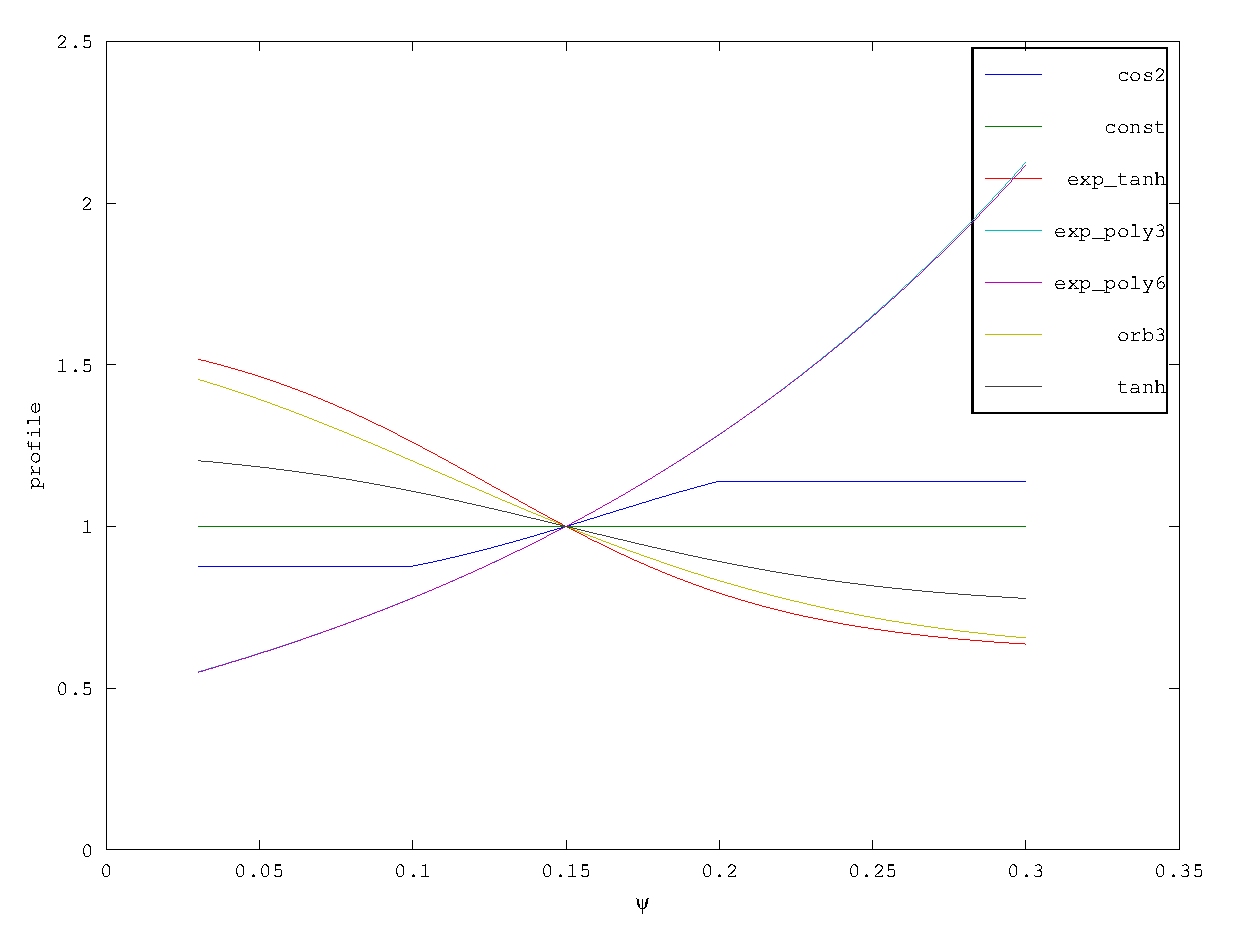
\includegraphics[width=0.8\textwidth]{comparisonProfile}
    \caption{\label{comparisonProfile}Comparsion of some possible profiles for density/temperature. All use the same set of parameters (see text) and thus might be nonphysical.}
  \end{center}
\end{figure}

\begin{figure}
  \begin{center}
    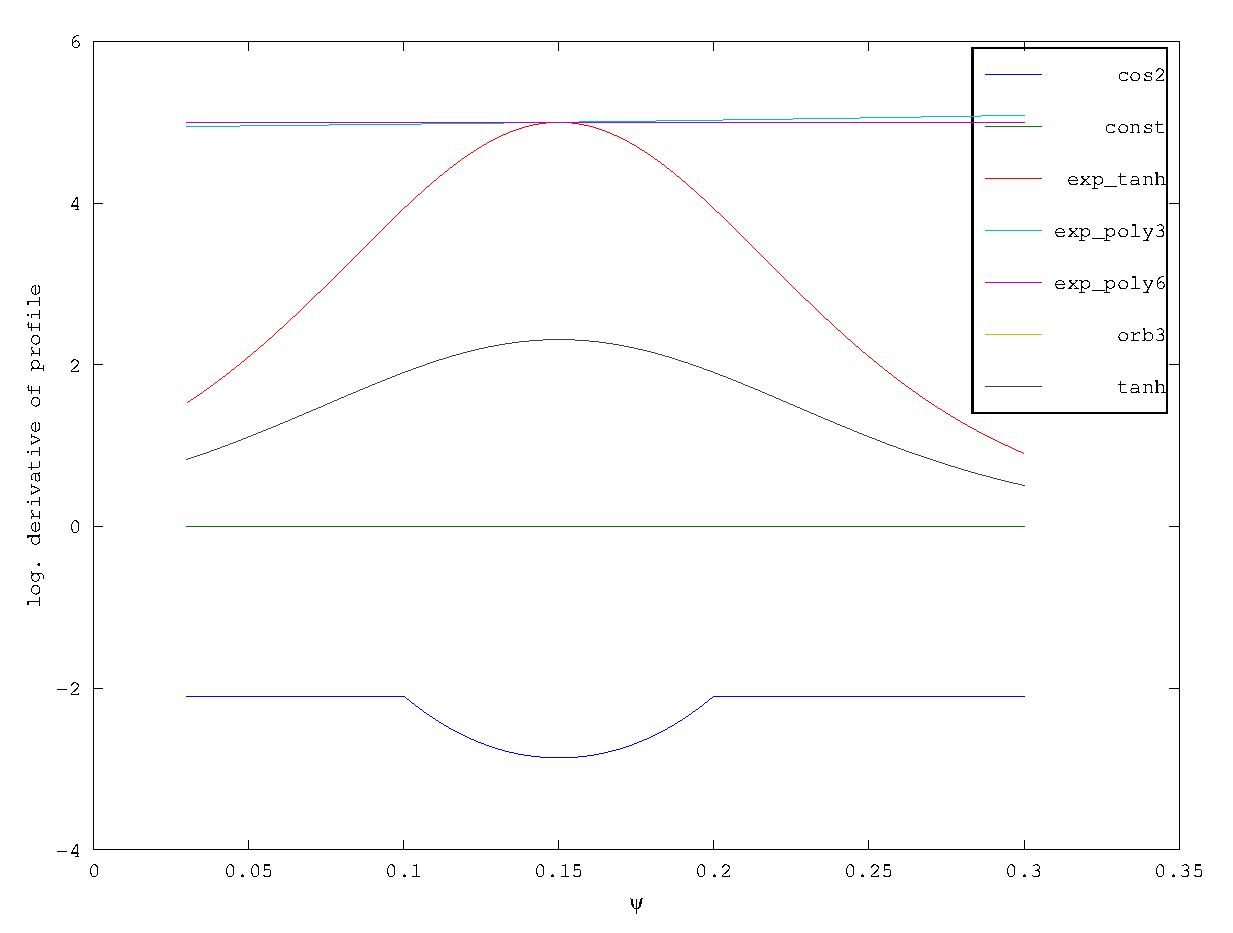
\includegraphics[width=0.8\textwidth]{comparisonDprofile}
    \caption{\label{comparisonDprofile}Comparsion the gradients length of some possible profiles for density/temperature. All use the same set of parameters (see text) and thus might be nonphysical.}
  \end{center}
\end{figure}

\begin{figure}
  \begin{center}
    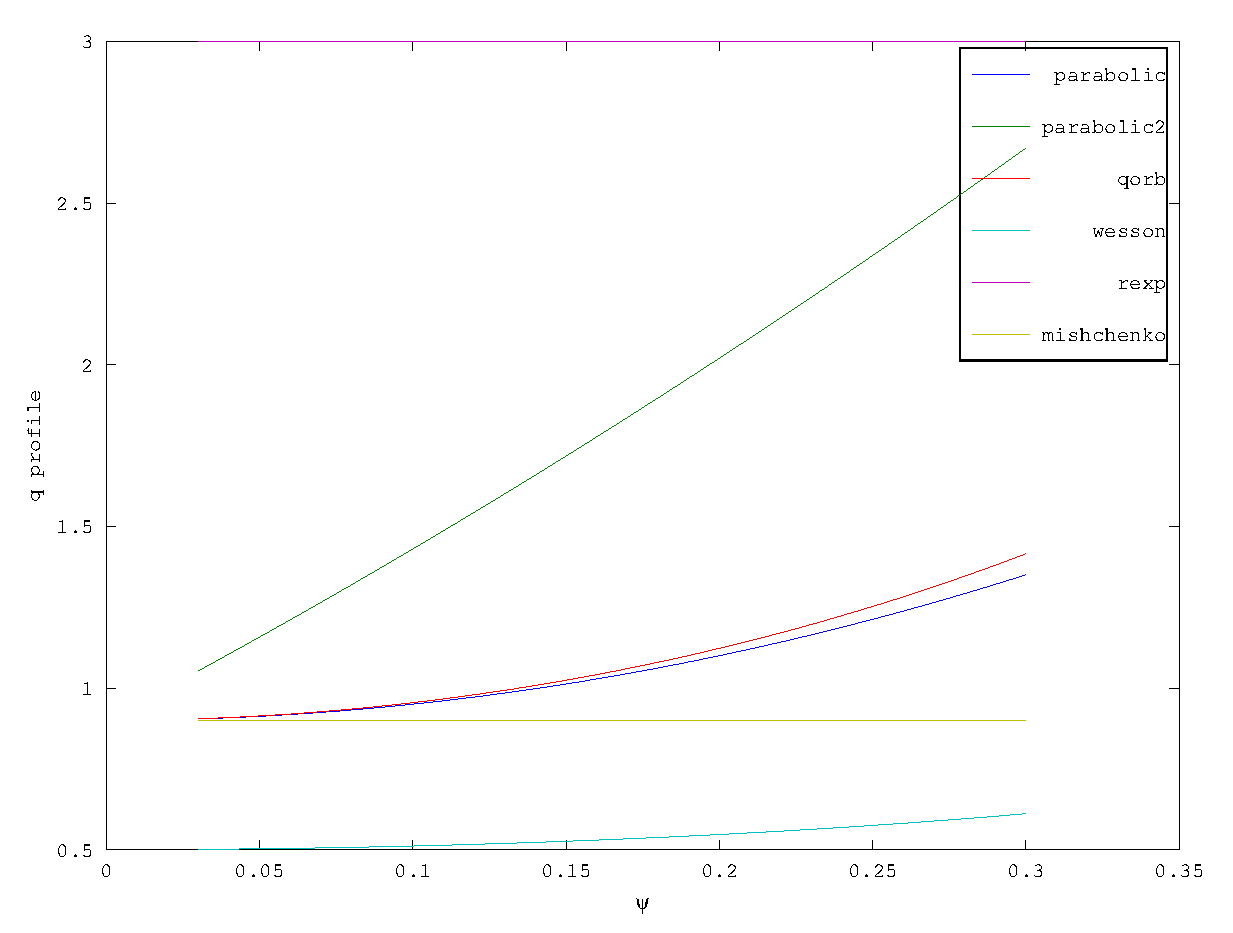
\includegraphics[width=0.8\textwidth]{comparisonQprofile}
    \caption{\label{comparisonQprofile}Comparison of some possible safety factor profiles. All use the same set of parameters (see text) and thus might be nonphysical.}
  \end{center}
\end{figure}

\begin{figure}
  \begin{center}
    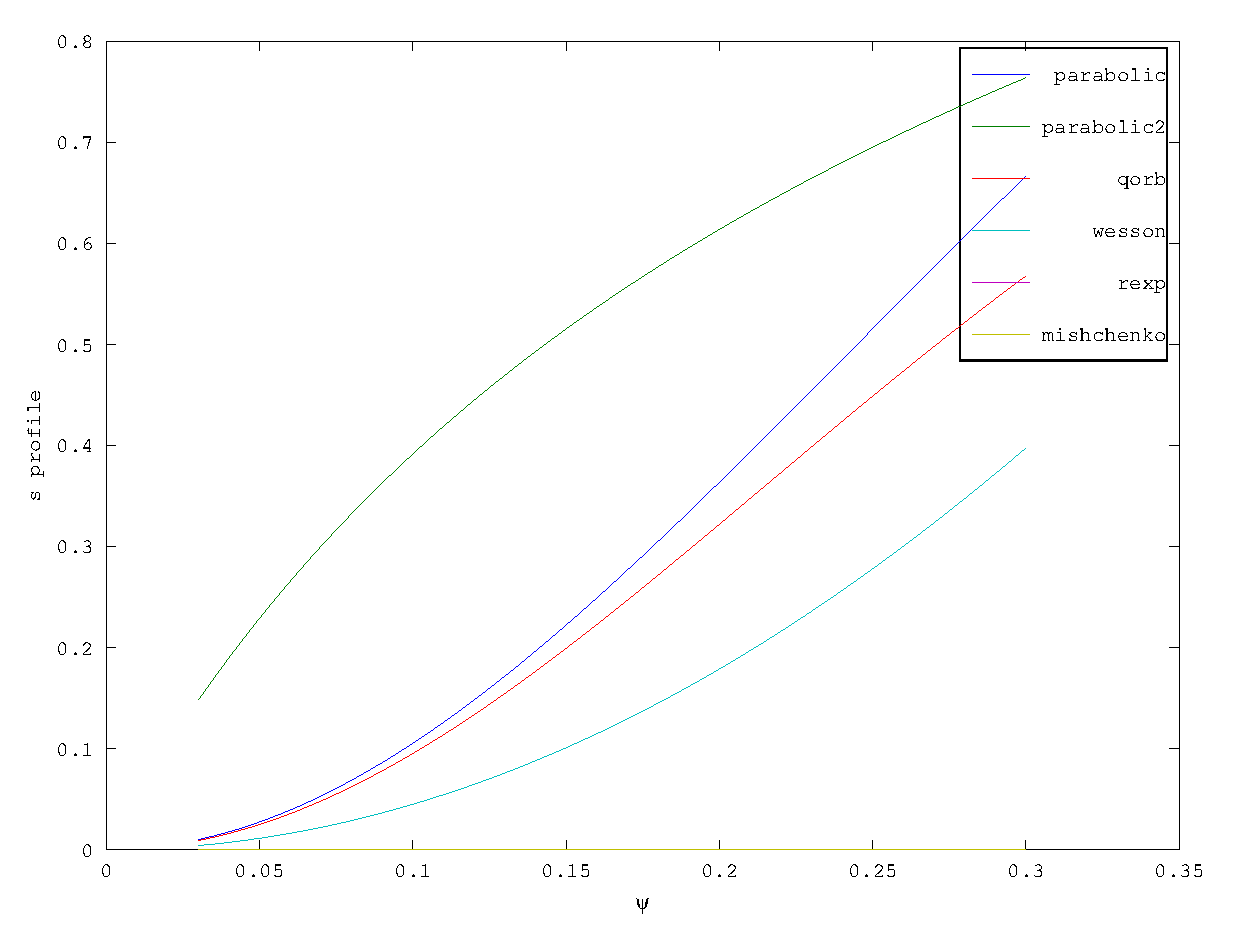
\includegraphics[width=0.8\textwidth]{comparisonSprofile}
    \caption{\label{comparisonSprofile}Comparison of the shear for some possible safety factor profiles. All use the same set of parameters (see text) and thus might be nonphysical.}
  \end{center}
\end{figure}


\subsection{Density/Temperature profile option: cosh2}
Allows to have a plateau like gradient profile, i.e. almost constant in the
middle and going to zero at the border.

\begin{eqnarray*}
G_0    = {\rm dens\_prof\_coef}(1)   &\hbox{the density / temperature at $x = X_0$} \cr
R/L_G  = {\rm dens\_prof\_coef}(2)   &\hbox{gradient length R/L_G at $x = X_0$}\cr
X_0    = {\rm dens\_prof\_coef}(3)   &\hbox{Radial location of the maximum gradient}\cr
w      = {\rm dens\_prof\_coef}(4)   &\hbox{the normalized width of the plateau $\Delta x / R_0$}\cr
\Delta = {\rm dens\_prof\_coef}(5)   &\hbox{Width that determines the rise of the $R/L_T$ profile}
\end{eqnarray*}
\begin{equation}
X = {\rm min}({\rm max}(X_0-w/2,\psi),X_0+w/2.)  
\end{equation}
\begin{equation}
G = G_0 \exp\biggl [ -\frac{R }{ L_G} (X-X_0) + \frac{R}{ L_G} \Delta \tanh \biggl ( \frac{X - X_0 + w / 2 }{ 
\Delta} \biggr ) + \frac{R}{ L_G} \Delta \tanh \biggl ( \frac{X - X_0 - w / 2 }{ 
\Delta} \biggr ) \biggr ] 
\end{equation}
\begin{equation}
G^\prime = \frac{R}{ L_G} \biggl ( 1 - \frac{1 }{ \cosh^2 ((X - X_0 + w / 2)/\Delta)} - 
 \frac{1 }{ \cosh^2 ((X - X_0 - w / 2)/\Delta)}\biggr ) 
\end{equation}
\begin{equation}
G_{\rm norm} = G_0   
\end{equation}

\subsection{Density/Temperature profile option: 'const'} 

\begin{eqnarray*}
G_0    = {\rm dens\_prof\_coef}(1)   &\hbox{the density / temperature }
\end{eqnarray*} 
\begin{equation}
G = G_0 
\end{equation}
\begin{equation}
G^\prime = 0
\end{equation}
\begin{equation}
G_{\rm norm} = G_0 
\end{equation}

\subsection{Density/Temperature profile option: 'exp_tanh'}

\begin{eqnarray*}
G_0    = {\rm dens\_prof\_coef}(1)   &\hbox{the density / temperature at $x = X_0$} \cr
R/L_G  = {\rm dens\_prof\_coef}(2)   &\hbox{gradient length R/L_G at $x = X_0$}\cr
X_0    = {\rm dens\_prof\_coef}(3)   &\hbox{Radial location of the maximum gradient}\cr
w      = {\rm dens\_prof\_coef}(4)   &\hbox{the normalized width of the gradient profile $\Delta x / R_0$}\cr
\end{eqnarray*} 
\begin{equation}
G = G_0 \exp \biggl ( - \frac{R}{ L_G} w \tanh \biggl ( \frac{\psi-X_0 }{ w} \biggr ) \biggr ) 
\end{equation}
\begin{equation}
G^\prime = \frac{R }{ L_G} \frac{1 }{ \cosh^2 ((\psi-X_0)/w)}
\end{equation}
\begin{equation}
G_{norm} = G_0
\end{equation}

\subsection{Density/Temperature profile option: '1_m_exp_tanh'}
\begin{eqnarray*}
G_0    = {\rm dens\_prof\_coef}(1)   &\hbox{the density / temperature at $x = X_0$} \cr
R/L_G  = {\rm dens\_prof\_coef}(2)   &\hbox{gradient length R/L_G at $x = X_0$}\cr
X_0    = {\rm dens\_prof\_coef}(3)   &\hbox{Radial location of the maximum gradient}\cr
w      = {\rm dens\_prof\_coef}(4)   &\hbox{the normalized width of the gradient profile $\Delta x / R_0$}\cr
\end{eqnarray*}
\begin{equation}
G = 1 - G_0 \exp \biggl ( - \frac{R}{L_G} w \tanh \biggl ( \frac{\psi-X_0}{w} \biggr ) \biggr )
\end{equation}
\begin{equation}
G^\prime = \frac{R}{L_G} \frac{1}{\cosh^2 \frac{\psi-X_0}{w}}
\end{equation}
\begin{equation}
G_{norm} = 1 - G_0
\end{equation}

\subsection{Density/Temperature profile option: exp_poly3}

Results in a quadratic profile of the gradient length. Limiting cases of linear 
(for a = 0) and constant (for a=0 and b=0) are included. Some care has to be taken 
to get physical profiles. To get a gradient length that is positive over the whole range, 
the inequality $b^2 < 4a$ has to be fullfilled.
\begin{eqnarray*}
G_0    = {\rm dens\_prof\_coef}(1)   &\hbox{the density / temperature at $x = X_0$} \cr
R/L_G  = {\rm dens\_prof\_coef}(2)   &\hbox{gradient length R/L_G at $x = X_0$}\cr
X_0    = {\rm dens\_prof\_coef}(3)   &\hbox{Radial location of the maximum gradient}\cr
a      = {\rm dens\_prof\_coef}(4)   &\hbox{constant for the quadratic term}\cr
b      = {\rm dens\_prof\_coef}(5)   &\hbox{constant for the linear term}
\end{eqnarray*}
\begin{equation}
G = G_0  \exp \left[ - \frac{R }{ L_G} \left(  \frac{a}{3} (\psi - X_0)^3
+ \frac{b}{2} (\psi - X_0)^2  + (\psi - X_0) \right) \right]
\end{equation}
\begin{equation}
G^\prime = \frac{R }{ L_G} \left[ a (\psi - X_0)^2 + b (\psi - X_0) + 1 \right]
\end{equation}
\begin{equation}
G_{\rm norm} = G_0 
\end{equation}

\subsection{Density/Temperature profile option: exp_poly6}

Results in a fifth and third order term as well as a constant for the
gradient length.
\begin{eqnarray*}
G_0    = {\rm dens\_prof\_coef}(1)   &\hbox{the density / temperature at $x = X_0$} \cr
R/L_G  = {\rm dens\_prof\_coef}(2)   &\hbox{gradient length R/L_G at $x = X_0$}\cr
X_0    = {\rm dens\_prof\_coef}(3)   &\hbox{Radial location of the maximum gradient}\cr
a      = {\rm dens\_prof\_coef}(4)   &\hbox{constant for the fifth order term}\cr
b      = {\rm dens\_prof\_coef}(5)   &\hbox{constant for the third order term}
\end{eqnarray*}
\begin{equation}
G = G_0 \exp \left[ - \frac{R }{ L_G} \left(  \frac{a}{6} (\psi - X_0)^6
                                          + \frac{b}{4} (\psi - X_0)^4
                                          +             (\psi - X_0) \right) \right]
\end{equation}
\begin{equation}
G^\prime = \frac{R }{ L_G} \left[  a (\psi - X_0)^5
                           +     b (\psi - X_0)^3
                           + 1 \right]
\end{equation}
\begin{equation}
G_{\rm norm} = G_0
\end{equation}

\subsection{Density/Temperature profile option : orb} 

This produces profiles equivalent to one of the options used in ORB5 (NEMORB). 
The calculation is a little more involved because these orb profiles are 
defined as function of a different radial coordinate. 

\begin{eqnarray*}
G_0    = {\rm dens\_prof\_coef}(1)   &\hbox{the density / temperature at $x = X_0$} \cr
R/L_G  = {\rm dens\_prof\_coef}(2)   &\hbox{gradient length R/L_G at $x = X_0$}\cr
X_0    = {\rm dens\_prof\_coef}(3)   &\hbox{Radial location of the maximum gradient}\cr
w      = {\rm dens\_prof\_coef}(4)   &\hbox{Width of the profile}\cr
X_e    = {\rm dens\_prof\_coef}(5)   &\hbox{minor radius of the plasma edge $X_e = a /R_0$}
\end{eqnarray*}
The values of $\bar {q}$ as used in ORB at the edge and in the centre 
\begin{equation} q_a = q(a) \sqrt{1 - X_e^2} \end{equation}
\begin{equation} q_0    = q(0) \end{equation}
Rescale the gradient length to have exactly the input value at the $s_0$ 
coordinate used in ORB
\begin{equation}
\frac{R}{ L_{G*}} = \frac{R/L_G }{ 1 - 1 / \cosh^2(X_0/w)} 
\end{equation}
Calculate the $s$ coordinate used in ORB 
\begin{equation} 
s = \sqrt{\left ( \frac{\log(1 + (q_a - q_0)\psi^2/(q_0 X_e^2)) }{ 
\log(1 + (q_a - q_0)/ q_0 )} \right ) }
\end{equation}
\begin{equation}
D(X) = \exp \left ( \frac{R }{ L_{G*}} \frac{s^2 }{ \cosh(x_0/w)^2} - 2\frac{R }{ L_{G*}} 
s w \tanh \left ( \frac{s - X_0 }{ w} \right ) \right ) 
\end{equation}
\begin{equation}
G(\psi) = G_0 D(\psi) / D(X_0) 
\end{equation}
\begin{equation}
G^\prime = \frac{R }{ L_{G*}} \left ( \frac{1 }{ \cosh^2((s-X_0)/w)} - 
\frac{1 }{ \cosh^2(x_0/w) } \right ) 
\end{equation}
\begin{equation}
G_{\rm norm} = G_0 
\end{equation}
  
\subsection{Density/Temperature profile option: 'orb3'}

One of the profiles used in ORB (NEMORB) 
\begin{eqnarray*}
G_0    = {\rm dens\_prof\_coef}(1)   &\hbox{the density / temperature at $x = X_0$} \cr
R/L_G  = {\rm dens\_prof\_coef}(2)   &\hbox{gradient length R/L_G at $x = X_0$}\cr
X_0    = {\rm dens\_prof\_coef}(3)   &\hbox{Radial location of the maximum gradient}\cr
w      = {\rm dens\_prof\_coef}(4)   &\hbox{Width of the profile}\cr
\Delta = {\rm dens\_prof\_coef}(5)   &\hbox{width that determines the rise of the profile}
\end{eqnarray*}
%\begin{equation}
%X = {\rm min}({\rm max}(\psi,X_0-w/2),X_0+w/2)
%\end{equation}
\begin{equation}
G = G_0 \exp \left ( - \frac{1}{2}\frac{R }{ L_G} \Delta \log \left ( 
\frac{\cosh((X - X_0 + w )/ \Delta) }{ \cosh((X-X_0-w)/\Delta) } \right ) \right)
\end{equation}
\begin{equation}
G^\prime = \frac{1}{2} \frac{R}{ L_G} \left ( \tanh \left ( \frac{X-X_0+w}{ \Delta} \right) 
- \tanh \left ( \frac{X - X_0 - w }{ \Delta} \right ) \right) 
\end{equation}
\begin{equation}
G_{\rm norm} = G_0 
\end{equation}
  

\subsection{Density/Temperature profile option: 'tanh'}
Profile is Taylor approximation of orb3, the gradient is chosen to be the same?\\
The tanh profile 
\begin{eqnarray*}
G_0    = {\rm dens\_prof\_coef}(1)   &\hbox{the density / temperature at $x = X_0$} \cr
R/L_G  = {\rm dens\_prof\_coef}(2)   &\hbox{gradient length R/L_G at $x = X_0$}\cr
X_0    = {\rm dens\_prof\_coef}(3)   &\hbox{Radial location of the maximum gradient}\cr
w      = {\rm dens\_prof\_coef}(4)   &\hbox{Width of the profile}\cr
\Delta = {\rm dens\_prof\_coef}(5)   &\hbox{width that determines the rise of the profile}
\end{eqnarray*}
\begin{equation}
G = G_0 \left[ 1.- \frac{\Delta}{2}\frac{R }{ L_G} \left ( \log \left (\cosh \left (\frac{\psi-X_0+w/2}{ 
\Delta} \right ) \right) - \log \left ( \cosh \left (\frac{\psi-X_0-w/2}{ \Delta} \right ) \right ) \right ) 
\right ] 
\end{equation}
\begin{equation}
G^\prime = \frac{1}{2} \frac{R }{ L_G} \left ( \tanh \left ( \frac{\psi-X_0+w/2)}{ \Delta} \right ) -  
\tanh \left ( \frac{\psi-X_0-w/2}{ \Delta} \right )  \right )
\end{equation}
The norm is the value of the profile at $X_0$, not the $G_0$ value (which should be equal to $G_0$)
\begin{equation}
G_{\rm norm} = G(X_0) 
\end{equation}

\subsection{q-profile option: parabolic} 

Parabolic q-profile 
\begin{eqnarray*}
q_0    = {\rm qprof\_coef}(1)   &\hbox{$q$ value at the axis} \cr
a      = {\rm qprof\_coef}(2)   &\hbox{coefficient for the quadratic term}
\end{eqnarray*}
\begin{equation}
q = q_0 + a \psi^2 
\end{equation}
with $\psi = r /R_0$ in circular geometry. 
\begin{equation}
\hat s = \frac{ 2 a \psi^2 }{ q_0 + a \psi^2} 
\end{equation}

\subsection{q-profile option: parabolic2} 

Second degree polynomial 
\begin{eqnarray*}
q_0    = {\rm qprof\_coef}(1)   &\hbox{$q$ value at the axis} \cr
a      = {\rm qprof\_coef}(2)   &\hbox{coefficient for the linear term}\cr
b      = {\rm qprof\_coef}(3)   &\hbox{coefficient for the quadratic term}
\end{eqnarray*}

\begin{equation}
q = q_0 + a \psi + b \psi^2 
\end{equation}
\begin{equation}
\hat s = \frac{a \psi + 2 b \psi^2}{q}
\end{equation}

\subsection{q-profile option: orb} 

For circular geometry one of the options in ORB is 
\begin{eqnarray*}
q_0    = {\rm qprof\_coef}(1)   &\hbox{$q$ value at the axis} \cr
a      = {\rm qprof\_coef}(2)   &\hbox{coefficient for the quadratic term}
\end{eqnarray*}
\begin{equation}
q = \frac{q_0 + a \psi^2}{\sqrt{1 - \psi^2}} 
\end{equation}
\begin{equation}
\hat s = \frac{2 a \psi^2 }{ q_0 + a \psi^2} - \frac{\psi^2 }{ 1 - \psi^2} 
\end{equation}

\subsection{q-profile option: wesson} 

The q-profile used in Wesson. For this profile $qprof_coef(1) \psi^2 < 1$ has to hold
over the entire profile, otherwise the term in the logarithm gets negative. 
If this happens, the simulation will abort.
\begin{eqnarray*}
D_w    = {\rm qprof\_coef}(1)   &\hbox{The aspect ratio squared}  (R/a)^{2} \cr
\nu    = {\rm qprof\_coef}(2)   &\hbox{Exponent of the q-profile.}\cr
q_0    = {\rm qprof\_coef}(3)   &\hbox{q value on the axis}\cr
\end{eqnarray*}
\begin{equation}
q = \frac{q_0 \psi^2 D_w }{ 1 - \exp((\nu+1)\log(1 - D_w \psi^2)) } 
\end{equation}
\begin{equation}
\hat s = 2 \left (1 - \frac{q(\nu + 1)}{q_0}\exp\left ( \nu \log(1-D_w \psi^2) \right) \right)
\end{equation}

\subsection{q-profile option: rexp} 

Exponential q-profile, with a cut off $q_c$. Values of the exponent lower than 
$q_c$ are set to $q_c$ with the shear then set to zero. 
\begin{eqnarray*}
a      = {\rm qprof\_coef}(1)   &\hbox{1/length for exponential increase } \cr
q_v    = {\rm qprof\_coef}(2)   &\hbox{Multiplication factor}\cr
q_c    = {\rm qprof\_coef}(3)   &\hbox{Cut off value}
\end{eqnarray*}
\begin{equation}
q = {\rm max}(q_v \psi \exp(a \psi),q_c) 
\end{equation}
\begin{equation}
\hat s = 1 + \psi a \quad \hbox{for $q>q_c$} 
\end{equation}

\subsection{q-profile option: mishchenko} 

This has for example been used in Mishchenko and Zocco, Phys. Plasmas 19. 
\begin{eqnarray*}
q_0      = {\rm qprof\_coef}(1)   &\hbox{The q-value on the axis} \cr
a        = {\rm qprof\_coef}(2)   &\hbox{Norm factor for $\psi$}\cr
\nu      = {\rm qprof\_coef}(3)   &\hbox{Exponent}
\end{eqnarray*}
\begin{equation}
q = q_0 + (1 - q_0) (\psi/ a)^\nu
\end{equation}
\begin{equation}
\hat s = \frac{\nu (1 - q_0) (\psi / a)^\nu }{ q} 
\end{equation}

\subsection{q-profile option: file} 

By specifying \name{prof_type='file'}, the $q$-profile is read from the file '\name{input.prof}'.
The block of geometry data in the file '\name{input.prof}' must be preceeded by a line starting with the text \verb|#Geometry|.
If Miller geometry is chosen, the data is expected to be given in 13 columns and \name{n_x_grid} rows.
The quantities in each row are \name{xgr},\name{qx},\name{shatx},\name{kappax},\name{deltax},\name{squarex},\name{ skappax},\name{sdeltax},\name{ssquarex},\name{Zmilx},\name{dRmilx},\name{dZmilx},\name{gradpx}, in this order.
\begin{verbatim}
#Geometry
  0.01022949   1.26822967   0.01021214   1.29296310   0.00248834  -0.00528476   0.00009362   0.00247875  -0.00003630   0.03824134  -0.00964105  -0.00147389   0.00000000
  0.01068848   1.26882114   0.01104428   1.29296896   0.00260034  -0.00528594   0.00010279   0.00259195  -0.00004001   0.03824021  -0.01007150  -0.00154127   0.00000000
  0.01114746   1.26943302   0.01189906   1.29297521   0.00271252  -0.00528711   0.00011236   0.00270567  -0.00004393   0.03823903  -0.01050195  -0.00160874   0.00000000
  0.01160645   1.27006485   0.01277532   1.29298176   0.00282480  -0.00528831   0.00012233   0.00281975  -0.00004801   0.03823780  -0.01093237  -0.00167609   0.00000000
...
\end{verbatim}
Otherwise, the data is expected to be given in 3 columns and \name{n_x_grid} rows.
The quantities in each row are \name{xgr},\name{qx},\name{shatx}, in this order.
\begin{verbatim}
#Geometry
  0.01022949   1.26822967   0.01021214
  0.01068848   1.26882114   0.01104428
  0.01114746   1.26943302   0.01189906
  0.01160645   1.27006485   0.01277532
...
\end{verbatim}




% related to auctex mode and latex-preview-mode in Emacs:
%%% Local Variables:
%%% mode: latex
%%% TeX-master: "doc"
%%% End:
